
    \documentclass[tikz,convert={outfile=\jobname.png}]{standalone}
    \usetikzlibrary{mindmap,trees,backgrounds}
    \usepackage{fontspec}
    \defaultfontfeatures{Ligatures=TeX,Scale=3}
    \setmainfont{M+ 1mn}
    
    
    \definecolor{tiffanyblue}{RGB}{10.200000000000001, 186.15, 181.04999999999998}
    \definecolor{tigerseye}{RGB}{224.4, 140.25, 61.199999999999996}
    \definecolor{utahcrimson}{RGB}{211.64999999999998, 0.0, 63.75}
    \definecolor{palatinatepurple}{RGB}{104.55, 40.800000000000004, 96.9}
    \definecolor{oxfordblue}{RGB}{0.0, 33.15, 71.4}
    \definecolor{dandelion}{RGB}{239.7, 224.4, 48.45}
    \definecolor{pumpkin}{RGB}{255.0, 117.30000000000001, 22.95}
    \definecolor{white}{RGB}{255.0, 255.0, 255.0}
    \definecolor{dimgray}{RGB}{104.55, 104.55, 104.55}
    
    \begin{document}
    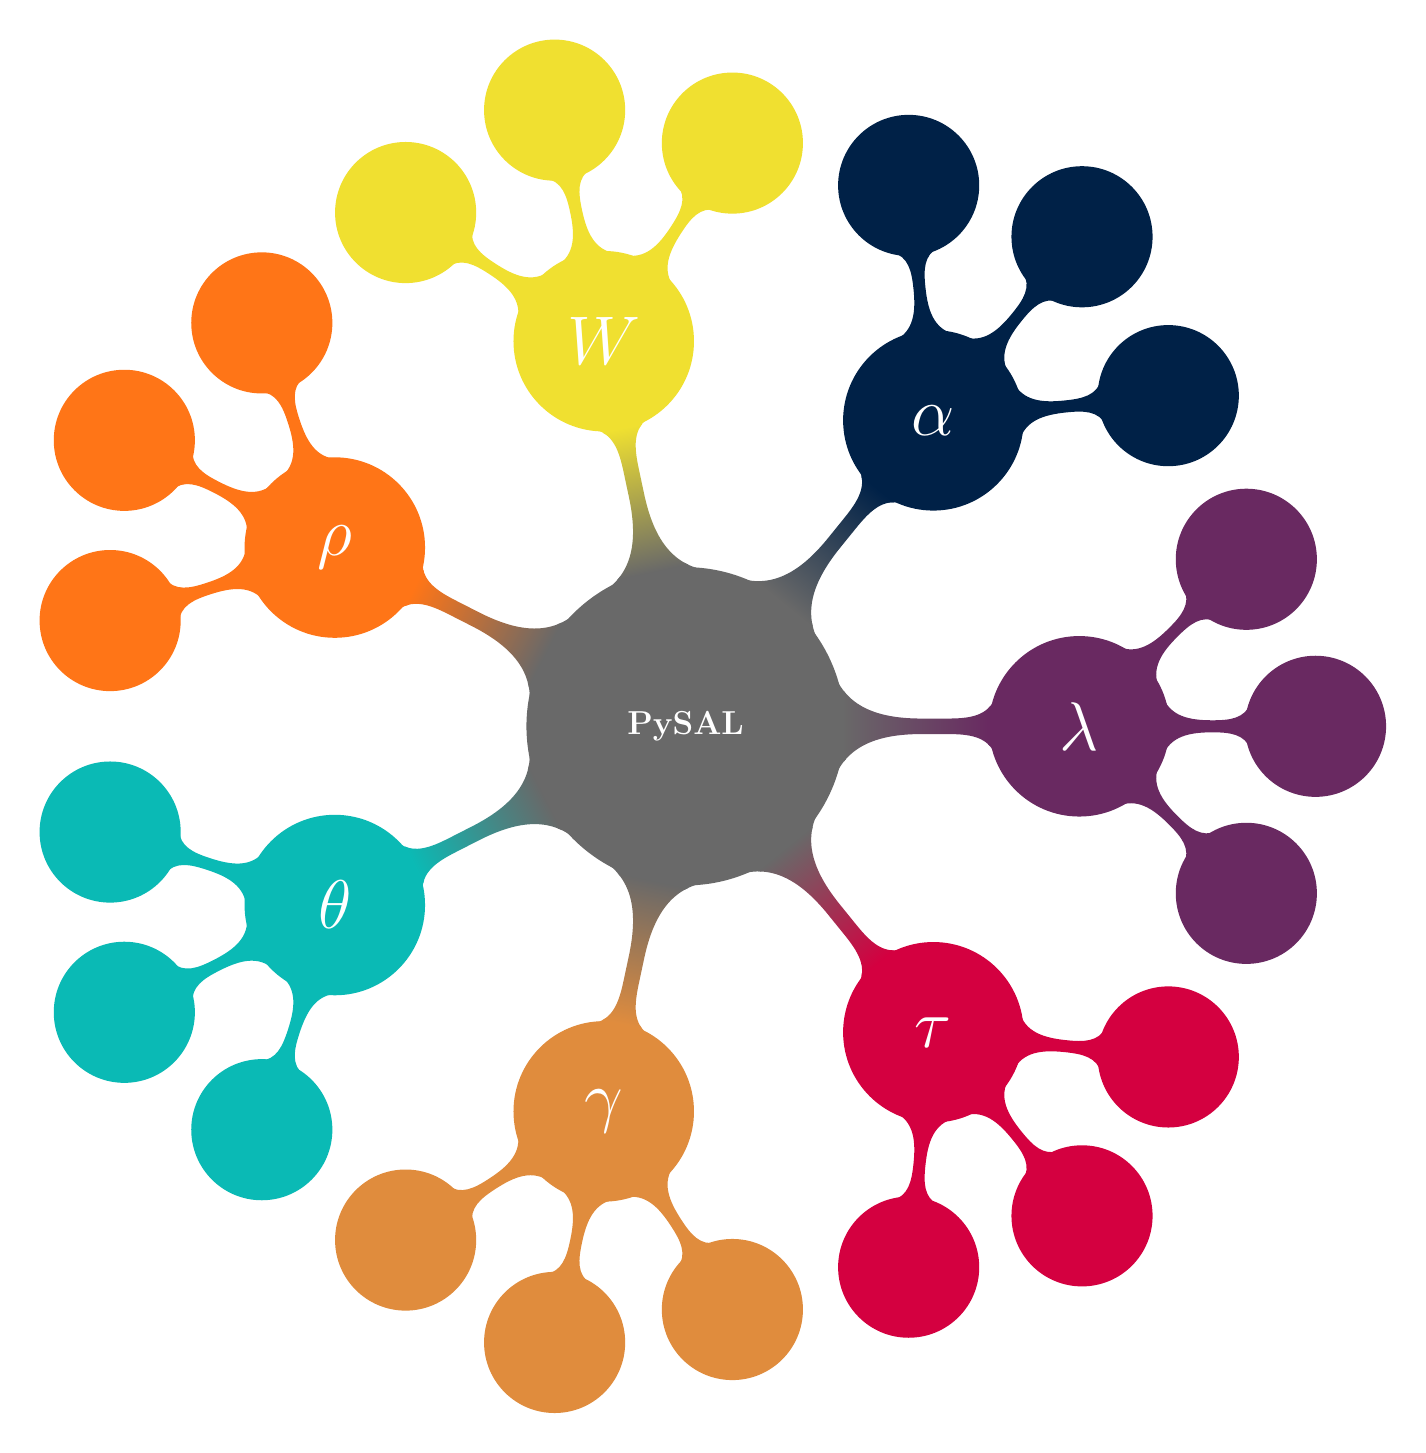
\begin{tikzpicture}[
        background rectangle/.style={fill=white},
        show background rectangle,
        mindmap,
        grow cyclic,
        every node/.style=concept,
        concept color=dimgray,
        text=white,
        level 1/.append style={
            level distance=5cm,
            sibling angle=51,
            font=\Huge
        },
        level 2/.append style={
            level distance=3cm,
            sibling angle=45
        }
    ]
    
        \node[concept color=dimgray]{\large\bfseries{PySAL}}
        child [concept color=tiffanyblue]{ node {$\theta$}
            child { node { }}
            child { node { }}
            child { node { }}
         }
        child [concept color=tigerseye]{ node {$\gamma$}
            child { node { }}
            child { node { }}
            child { node { }}
         }
        child [concept color=utahcrimson]{ node {$\tau$}
            child { node { }}
            child { node { }}
            child { node { }}
         }
        child [concept color=palatinatepurple]{ node {$\lambda$}
            child { node { }}
            child { node { }}
            child { node { }}
         }
        child [concept color=oxfordblue]{ node {$\alpha$}
            child { node { }}
            child { node { }}
            child { node { }}
         }
        child [concept color=dandelion]{ node {$W$}
            child { node { }}
            child { node { }}
            child { node { }}
         }
        child [concept color=pumpkin]{ node {$\rho$}
            child { node { }}
            child { node { }}
            child { node { }}
         }
                ;
    \end{tikzpicture}
    \end{document}